\documentclass{article}
\usepackage{graphicx} % Required for inserting images
\usepackage[utf8]{inputenc}
\usepackage[english]{babel}
\usepackage[tablegrid,nochapter]{vhistory} %%Vhistory simplifies the creation of a history of versions of a document
\usepackage[nottoc]{tocbibind} %%Automatically adds the bibliography and/or the index and/or the contents, etc., to the Table of Contents listing
\usepackage{authblk}
\usepackage{float}
\usepackage[raggedrightboxes]{ragged2e}


% Margins
\topmargin=-0.45in
\evensidemargin=0in
\oddsidemargin=0in
\textwidth=6.5in
\textheight=9.0in
\headsep=0.25in

\counterwithin{table}{subsection}

\def\BoldTitle{Követelményelemzés}
\def\Subtitle{Élő LEGO Projekt Irányításához\\}

\title{\textbf{\BoldTitle}\\\Subtitle}

\author{\textsc{\Large Projektvezető: Németh Gábor Árpád} \\ \textsc{Csapat tagjai:} Habzda Fruzsina Mária Horváth Sára, Kemény Dániel, Kiss Ámon, Novák Lilla, Racskó Balázs, Székely Szilárd, Torvinen Aili, Tóth Dóra, Vágó Blanka}

\date{\today}

\begin{document}

\maketitle

\pagebreak
\tableofcontents % Inhaltsverzeichnis

\pagebreak
\section{Revision History}

\begin{versionhistory}
    \vhEntry{1.0}{2023. November 3.}{Habzda Fruzsina Mária}{Első vázlat}
    \vhEntry{1.1}{2023. November 23.}{Novák Lilla}{A vázlat kibővítése és részekre osztása}
\end{versionhistory}


\pagebreak
\section{Projekt bemutatása}

(összefoglaló ezekről, kb 1 oldal;
miről szól a projekt?
kinek a számára készül?
ki a kivitelező?
mik a kritériumok?
miért készül a projekt, miért van szükség rá?
mi a célja?
időtartam, költségvetés
rizikók)


\begin{itemize}
\item felsorolás1
\item felsorolás2
\end{itemize}


\pagebreak
\section{Követelmények}

követelmények számozása és felépítése (hogyan épül fel egy azonosító; követelménycsoport-id)
a megvalósítás fázisai (fázisok felsorolása, rövid leírása, követelményeik, időtartama) 
XY1 követelmény csoport követelményei (követelmények táblázatos leírása, azonosító, leírás)
XY2 ...

\subsection{*programozási felületek*}

(valami bevezető szöveg az adott részhez)

\subsubsection{*programozóknak*}

(itt is valami bevezető szöveg az adott részhez)

\begin{table}[htbp]
\centering
\begin{tabular}{|c|p{14cm}|}
\hline
\textbf{Azonosító} & \textbf{Leírás}        \\ 
\hline
       azonosító1  & Lorem ipsum dolor sit amet, consectetur adipiscing elit. Fusce facilisis nibh non sapien consequat ultricies. Phasellus in dapibus mauris. Nam consectetur tempus posuere. Fusce luctus ac magna quis maximus. Donec a arcu porttitor, blandit orci quis, suscipit justo. Aliquam scelerisque lobortis ornare. Praesent vel lorem eget mi vehicula elementum. Fusce dignissim nisl ut sem lobortis gravida. Quisque non erat porta, maximus nisi sed, hendrerit enim. In sollicitudin sollicitudin tempor. Duis ut mattis tellus. Maecenas velit purus, ultrices quis accumsan eu, interdum quis urna. In hac habitasse platea dictumst. Fusce ornare lectus orci, ut imperdiet ligula efficitur vel. Cras condimentum est a blandit fermentum. Nam placerat lobortis risus, non cursus magna tempor in. Donec fringilla posuere eros eget tristique. \\
\hline
\end{tabular}
\caption{táblázat leírása}
\label{table:my_label}
\end{table}

\subsubsection{Alkalmazás követelményei}

A fiatalabb korosztályt megcélzó alkalmazás felülete 5 fő részből fog állni, amelyek segítségével a felhasználók könnyen és hatékonyan dolgozhatnak:

\begin{itemize}
\item \textbf{Navigációs sáv:} 
Az oldal tetején elhelyezkedő menü segítséget nyújt a fájlok kezeléséhez, beleértve a mentést, betöltést és egyéb fájlalapú műveleteket, amelyek segítségével könnyedén lehet tárolni és visszatölteni a kész programokat.
\item \textbf{Munkaterület:}
A Munkaterület a fő területe a felületnek, ahol a felhasználók programjaikat építhetik, szerkeszthetik és megtekinthetik. Ide helyezhetik el a különböző programozási elemeket az eszköztárból, melyeket könnyedén lehet mozgatni, valamint összekapcsolni egymással.
\item \textbf{Beállítások:} 
A jobb oldalon elhelyezkedő panel lehetőséget nyújt az elemek részletes beállításaira. Itt állíthatók az elemek specifikus tulajdonságai és paraméterei, ami további testreszabást és funkcionalitást biztosít a programoknak.
\item \textbf{Eszköztár:}
A bal oldalon található panelon számos programozási elem, mint például ciklusok, elágazások, hangvezérlő modulok és vizuális elemek állnak rendelkezésre. Ezek az eszközök könnyen hozzáférhetőek és húzhatók a fő felületre a program építése során.
\item \textbf{Programkód megjelenítő:}
Az oldal alján, a Programkód megjelenítőben a felhasználók által összeállított programok jelennek meg C++ formátumban. Ez az ablak segít a felhasználóknak megérteni a programozás logikáját és struktúráját, miközben átlépnek a vizuális programozásról a kódolás gyakorlatába.
\end{itemize}

\begin{figure}[!h]
\centering
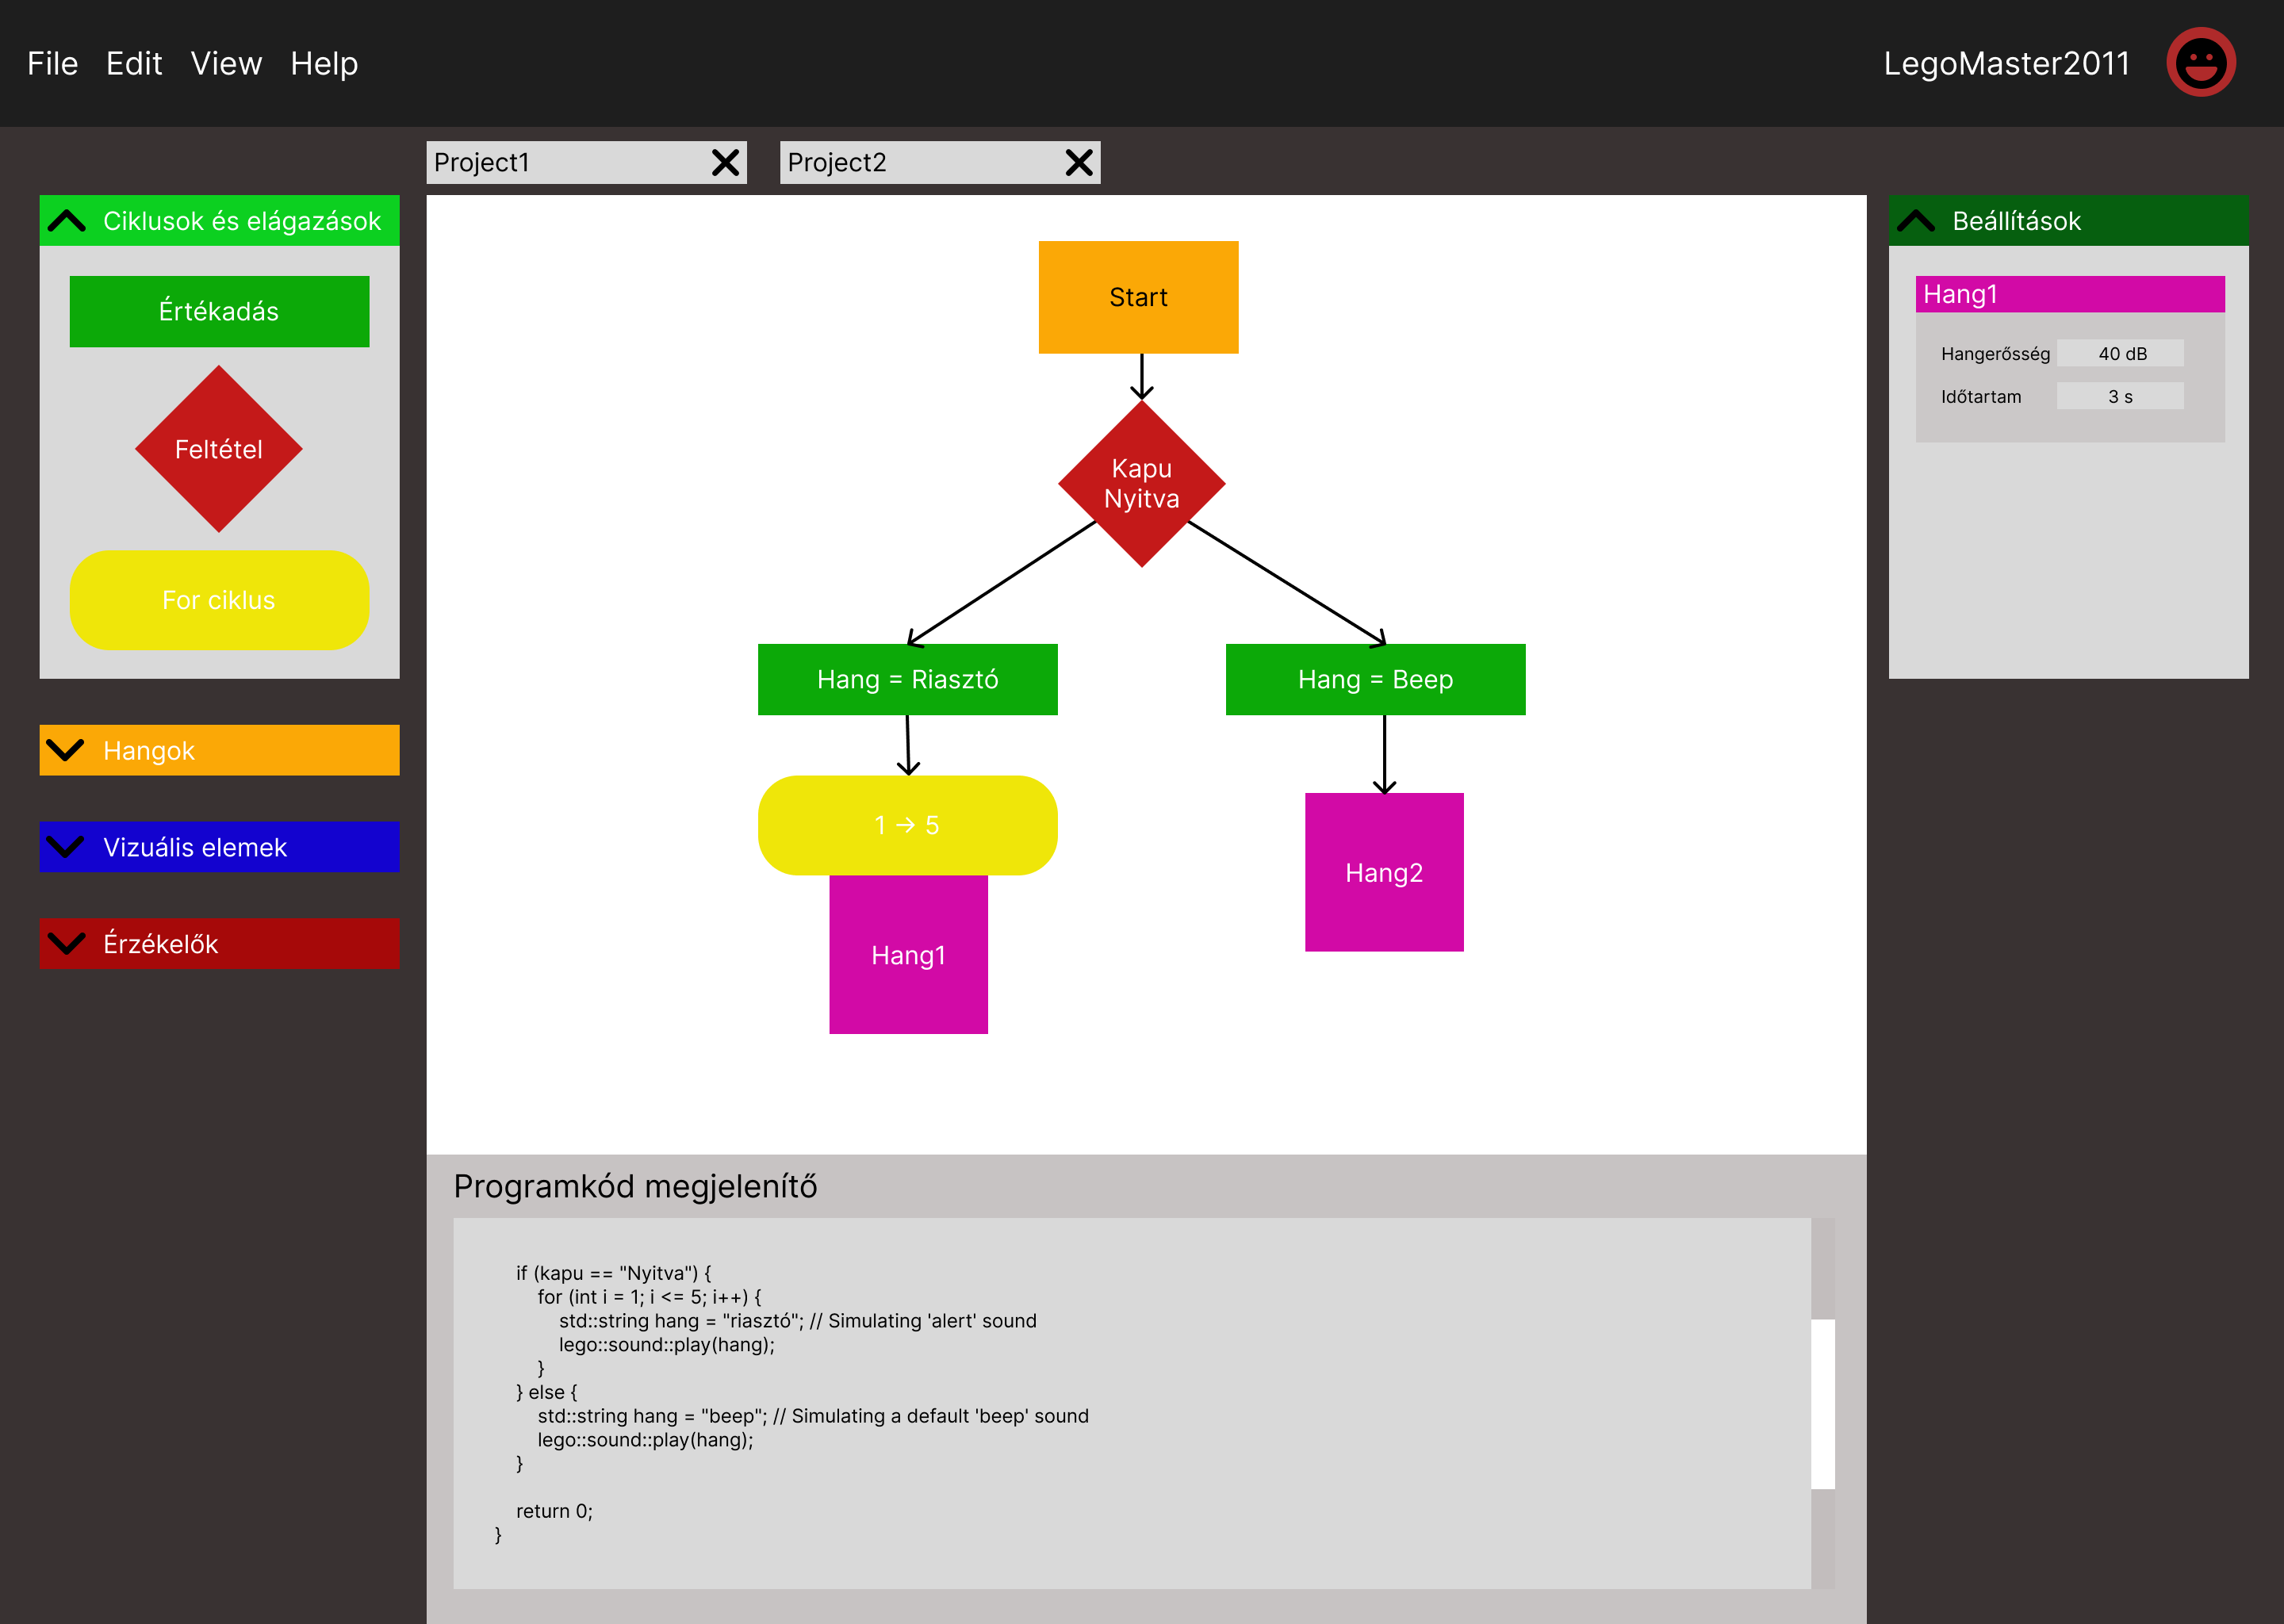
\includegraphics[width=1\linewidth]{gyerekeknek-felulet.png}
\caption{\label{fig:image}Gyerekeknek felület}
\end{figure}

\begin{table}[htbp]
\centering
\begin{tabular}{|c|p{14cm}|}
\hline
\textbf{Azonosító} & \textbf{Leírás}        \\ 
\hline
\textbf{A\_01} & Az alkalmazásnak lehetőséget kell biztosítania a lokális fájlok tárolására a vezérlőegységen belül, korlátozva a maximális 1GB tárhelyigényt. Későbbi fejlesztések során az alkalmazásnak támogatnia kell a fájlok megosztási lehetőségeit és a felhőalapú tárolást a további bővíthetőség érdekében \\\hline
\textbf{A\_02} & Az alkalmazásnak lehetőséget kell biztosítania a felhasználók számára a programjaik megosztására egy beépített fórum felületen keresztül. Ezen a fórumon a felhasználók megoszthatják saját kódjaikat, segítséget kérhetnek vagy értékeléseket adhatnak mások programjaira, lehetővé téve a közösségi tapasztalatok és segítségnyújtás megosztását a felhasználók között. \\\hline
\textbf{A\_03} & A programozói felületnek böngésző alapúnak kell lennie, támogatva a legelterjedtebb böngészőket: Chrome, Firefox, Safari, valamint Edge-t. Ennek révén biztosítva van a kompatibilitás és az optimális működés a felhasználók széles körű böngészőválasztéka esetén.\\\hline
\textbf{A\_04} & Az oldal tetején elhelyezkedő menürendszernek biztosítania kell a fájlok kezelését és egyéb fájlalapú műveleteket. Ennek részeként tartalmaznia kell olyan menüpontokat, mint a "File", "Edit", "View", "Help", valamint a jobb sarokban a felhasználó felhasználóneve. Ezek a menüpontok segítséget nyújtanak a fájlok mentéséhez, betöltéséhez és egyéb fájlalapú műveletek elvégzéséhez. \\\hline
\textbf{A\_05} & A jobb oldalon elhelyezkedő panel funkciójának ki kell terjednie az elemek részletes beállításaira. Ezen a felületen a felhasználóknak lehetőséget kell biztosítani arra, hogy az egyes elemek specifikus tulajdonságait és paramétereit testre szabhassák. Ennek révén a felhasználóknak képesnek kell lenniük részletesen finomhangolni az elemek működését és megjelenését, továbbá lehetőséget kell adni a funkcionalitás bővítésére a programokban. Az elemek részletes konfigurálhatósága növeli a rugalmasságot és segíti a felhasználókat az alkalmazásban való hatékonyabb és testreszabottabb munkavégzésben. \\\hline
\textbf{A\_06} & A bal oldalon található panelen elérhetőnek kell lennie a következő programozási elemeknek:
\begin{itemize}
    \item Ciklusok és elágazások
    \item Hangvezérlő modulok
    \item Vizuális elemek
    \item Érzékelők
\end{itemize}

Ezeknek az eszközöknek könnyen hozzáférhetőnek és használhatónak kell lenniük, ezért egy lenyíló listában kell elhelyezkedniük, lehetővé téve a felhasználók számára azok egyszerű húzását és elhelyezését a fő felületre a programok építése során.\\\hline

\textbf{A\_07} & A vizuális elemek alakzatok formájában jelennek meg és különböző színekkel rendelkeznek, hogy a gyerekek számára könnyen használható legyen. \\\hline
\textbf{A\_08} & Az oldal alján található Programkód megjelenítő felületen kell megjeleníteni a felhasználók által összeállított programokat C++ formátumban. Ez az ablak fontos szerepet tölt be azzal, hogy segítse a felhasználókat a programozás logikájának és struktúrájának megértésében, miközben átmennek a vizuális programozásból a kódolás gyakorlatába. A megjelenítő felületnek pontosan és érthetően kell bemutatnia a kódokat, hogy a felhasználók könnyen olvashassák, megérthessék és tanulhassanak belőlük a kódolási folyamat során.\\\hline

\textbf{A\_09} & A Munkaterületnek a fő részének kell lennie az alkalmazáson belül, ahol a felhasználók a programjaikat létrehozhatják, szerkeszthetik és megtekinthetik. Ide kell helyezni és rendezni a különböző programozási elemeket az eszköztárból, hogy a felhasználók könnyedén elhelyezhessék és mozgathassák azokat a Munkaterületen.\\\hline

\textbf{A\_10} & Az elemek közötti mozgatásnak és kapcsolatok kialakítása nyilak segítségével valósítandó meg, hogy egyszerű és intuitív legyen, hogy a felhasználók gördülékenyen és hatékonyan tudjanak dolgozni a programjaik létrehozásakor. \\\hline
\hline
\end{tabular}
\caption{Gyerekeknek szánt felület követelményei}
\label{table:my_label}
\end{table}

\subsection{*távirányítók*}
\subsubsection{*fizikai*}
\subsubsection{*app*}

\subsection{*weboldal*}
\subsubsection{*megosztás*}
\subsubsection{*dokumentáció*}


\pagebreak
\section{Szójegyzék}

(szavak csoportosítva, definíciókkal ellátva)


\end{document}